%! TEX root = **/000-main.tex
% vim: spell spelllang=en:

\section{Data exploration}%
\label{sec:data-exploration}

\subsection{Pre-processing}%
\label{sub:pre-processing}

\subsection{Missing values}%
\label{sub:missing-values}

Some columns had a lot of missing values. We decided to drop any column with
more than 20\% missing values. The rest of missing values were imputed using a
simple KNN imputation. \Cref{tab:missing-values} shows the number of imputed
values for each column. The columns with 130 missing values, correspond all to
the same 130 rows.

\begin{table}[htb]
  \centering
  \caption{Imputed Missing values}%
  \label{tab:missing-values}
  \begin{tabular}{llr}
    \toprule
    \textbf{Column} & \textbf{Description} & \textbf{Missing} \\
    \midrule
    \texttt{gs}          & Games Started               & 114 \\
    \texttt{orb\_per\_g} & Offensive Rebounds Per Game & 29  \\
    \texttt{drb\_per\_g} & Defensive Rebounds Per Game & 29  \\
    \texttt{sos}         & Strength of Schedule        & 130 \\
    \texttt{mp}          & Minutes Played              & 130 \\
    \texttt{tov\_pct}    & Turnovers Percentage        & 130 \\
    \texttt{ows}         & Offensive Wins              & 130 \\
    \texttt{dws}         & Defensive Wins              & 130 \\
    \texttt{ws}          & Win Shares                  & 130 \\
    \texttt{ws\_per\_40} & Win Shares Per 40 Minutes   & 130 \\
    \bottomrule
  \end{tabular}
\end{table}

\subsection{Feature selection/extraction}%
\label{sub:feature-selection}

\subsection{Principal Component analysis}%
\label{sub:pca}

\begin{figure}[H]
  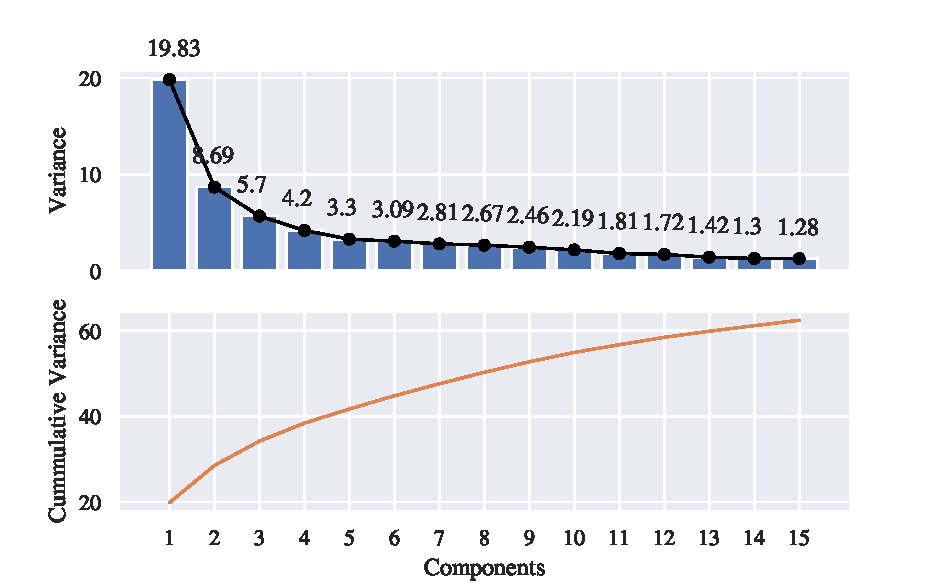
\includegraphics{pca_screeplot}
  \caption{Scree plot for PCA}%
  \label{fig:pca-scree}
\end{figure}

\begin{figure}[H]
  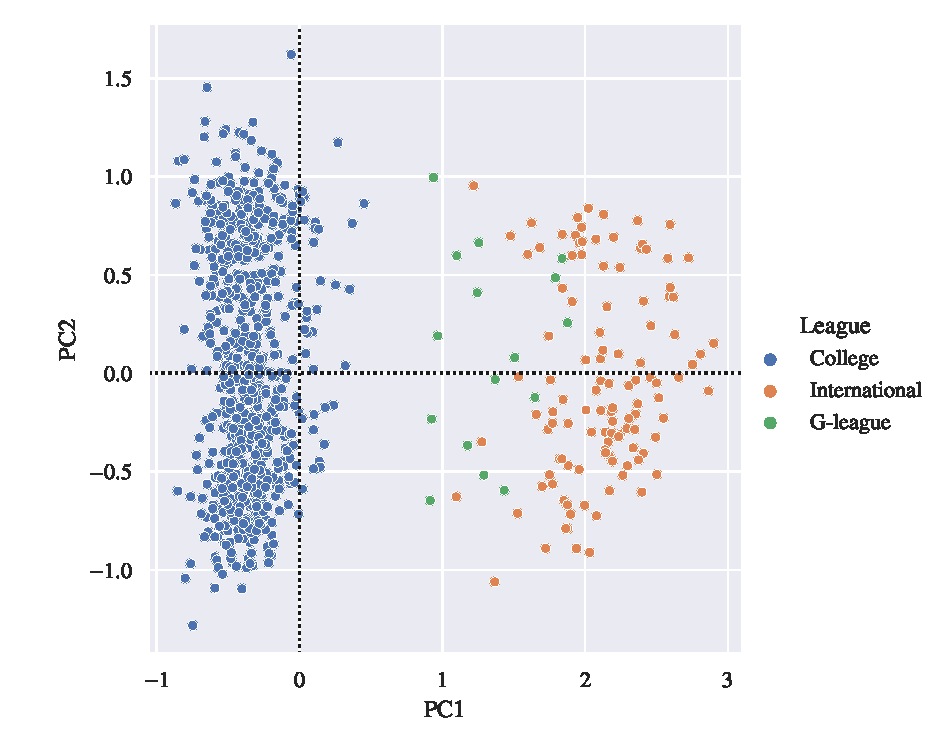
\includegraphics{pca}
  \caption{PCA projection}%
  \label{fig:pca}
\end{figure}

\subsection{Visualization}%
\label{sub:visualization}

\subsection{Clustering}%
\label{sub:clustering}

We experimented with several clustering algorithms and transformations on the data. We
found that the only meaningful Clusters we could identify were after scaling the data with
a min-max scaler and transforming it using PCA.
